% Created 2015-11-10 Tue 16:53
\documentclass[11pt]{article}
\usepackage[utf8]{inputenc}
\usepackage[T1]{fontenc}
\usepackage{fixltx2e}
\usepackage{graphicx}
\usepackage{longtable}
\usepackage{float}
\usepackage{wrapfig}
\usepackage{rotating}
\usepackage[normalem]{ulem}
\usepackage{amsmath}
\usepackage{textcomp}
\usepackage{marvosym}
\usepackage{wasysym}
\usepackage{amssymb}
\usepackage{hyperref}
\tolerance=1000
\author{Matthew Bregg}
\date{\today}
\title{cards}
\hypersetup{
  pdfkeywords={},
  pdfsubject={},
  pdfcreator={Emacs 24.5.1 (Org mode 8.2.10)}}
\begin{document}

\maketitle
\tableofcontents

\section{Card shape}
\label{sec-1}
\begin{itemize}
\item Rectangle, circle, etc
\item Corners, rounded, sharp?
\end{itemize}

\section{Decal}
\label{sec-2}

\begin{itemize}
\item Generic art, gets an art object
\item Decals will need to be patterned, one decal might want to be on each corner, or might want to go in a row, would be very awkward to have to manually do all this patterning : Decal shouldn't do patterning, let the transformation class do it.
\end{itemize}
\subsection{Decal types}
\label{sec-2-1}
\begin{itemize}
\item Image decals
\item Number decals
\item Text decals
\item Shape decal
\end{itemize}

\subsection{Nesting}
\label{sec-2-2}
Decals will want to be nested, a text box might want to be on top of a back ground.
\subsection{Layout class}
\label{sec-2-3}
Decorates an image with scale, position, etc, can be composited, and is clonable?
\begin{itemize}
\item Could then handle patterning
\item Composite
\end{itemize}

\subsubsection{Background}
\label{sec-2-3-1}
\begin{itemize}
\item Decal, covering the whole card
\end{itemize}

\subsubsection{General patterns}
\label{sec-2-3-2}
\begin{itemize}
\item Textbox
\item Border
\item Etc?
\end{itemize}
\section{Theming}
\label{sec-3}
\begin{itemize}
\item Sub decks
\item Some sets will have the same decal applied to the same spot
\item Others will have the same decal, but used in a different spot per card
\begin{itemize}
\item EX) Cards have some number of \$family decals, but those decals are in different spots, they don't know what image they are until we tell it its family. Thus, would say something like \$family = spades, and all the \$family decals will use the spades image.

\begin{verbatim}
clone =  prototype.clone();
clone.setDecal("family",spades);
\end{verbatim}
Families will still need per card information.
So perhaps\ldots{}
\begin{verbatim}
clone.setCharacter(charizard.jpg)
clone.setHP(120);
\end{verbatim}
\end{itemize}
\end{itemize}

\section{Cards}
\label{sec-4}
Card has a layout. Layouts can be cloned. 
Cards can be cloned.
\begin{itemize}
\item Card will have a name.
\item Card will have a layout
\item Card have a family? Family is just a map, string -> decal, Two types of layout leafs. FamilyLeaf, which just has a string, asks its family. DecalLeaf, which holds a decal.
\begin{itemize}
\item A family can be nested, will query its map, then parent map.
\end{itemize}
\end{itemize}

\section{Example UML}
\label{sec-5}

This should probably be split into multiple diagrams.
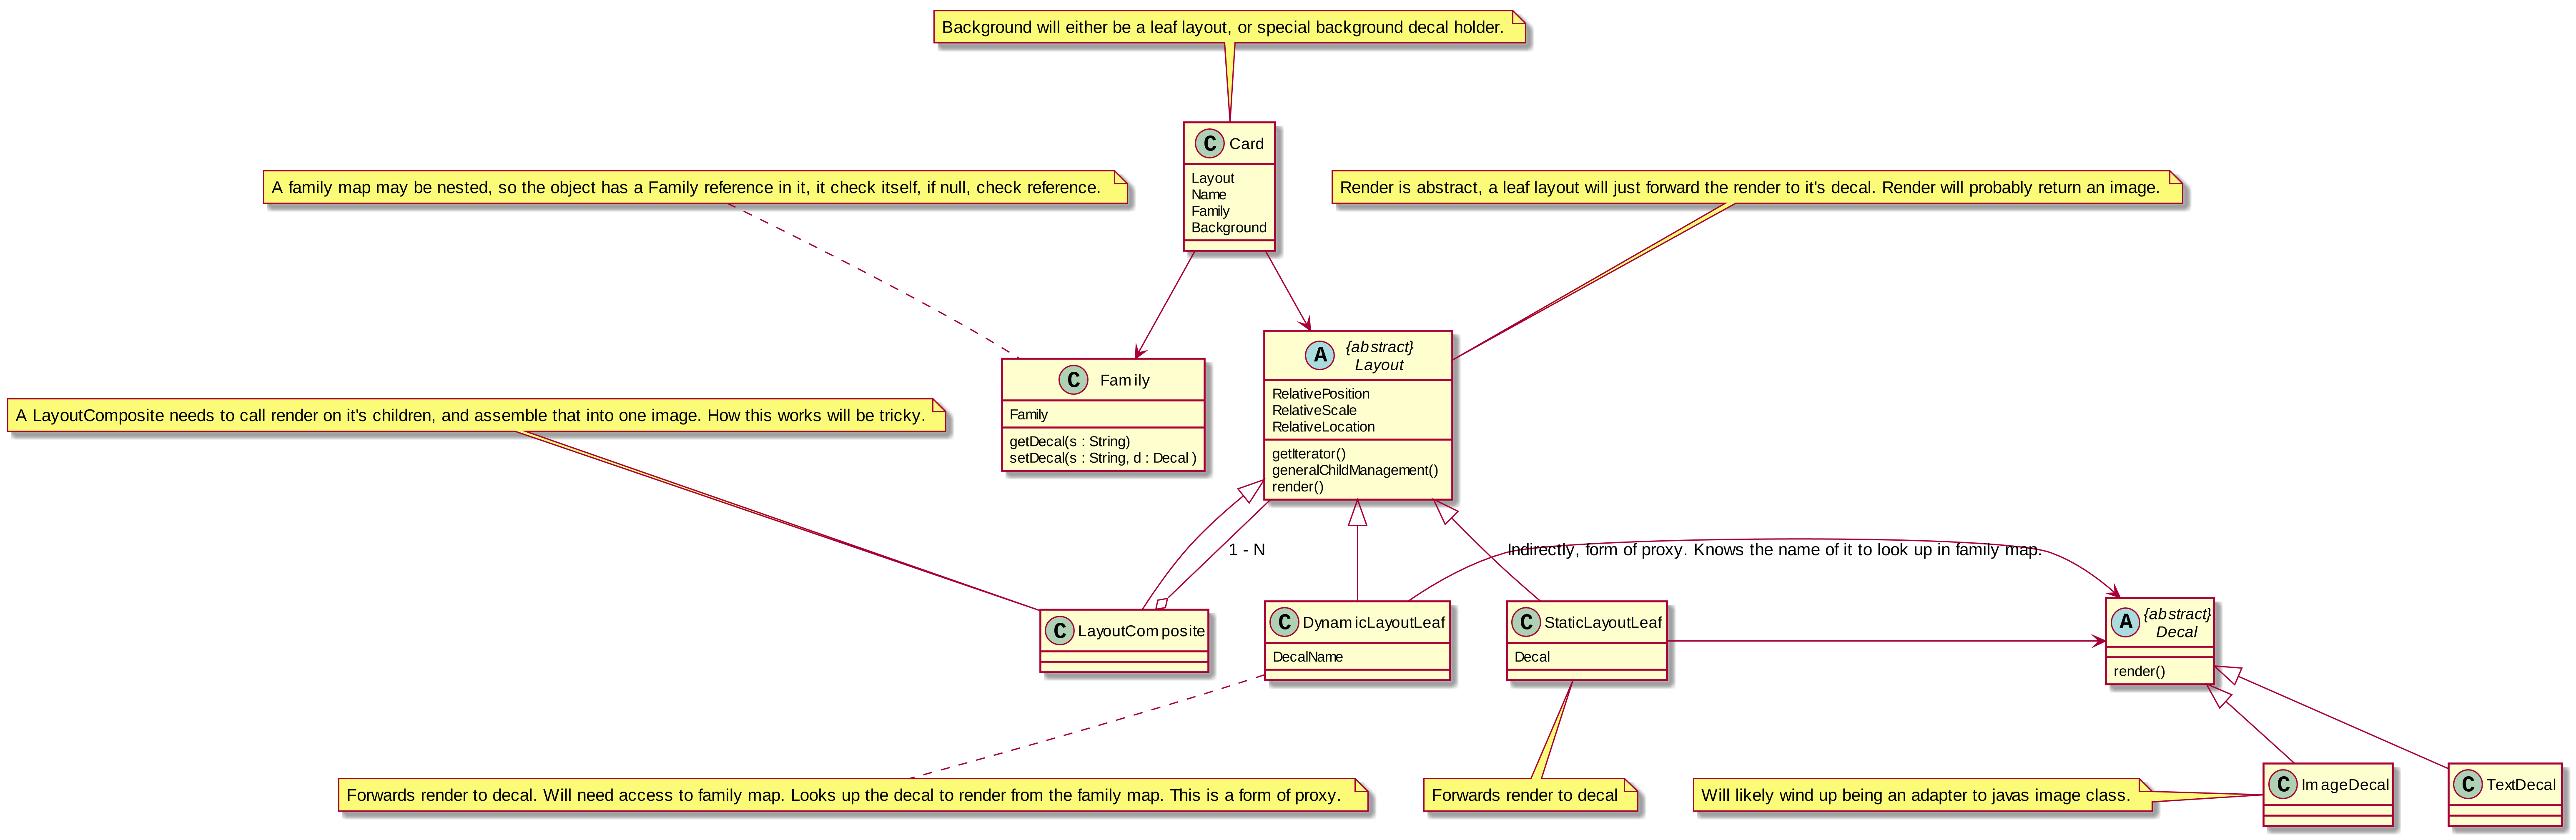
\includegraphics[width=.9\linewidth]{InitialCardsUmlqafd.png}
% Emacs 24.5.1 (Org mode 8.2.10)
\end{document}